\documentclass[11pt]{article}
\usepackage{enumerate}
\usepackage{tikz}
\usepackage{fullpage}
\usepackage{fancyhdr}
\usepackage{graphicx}

\usepackage{amsmath, amsfonts, amsthm, amssymb}
\setlength{\parindent}{0pt}
\setlength{\parskip}{5pt plus 1pt}
\pagestyle{empty}

\def\indented#1{\list{}{}\item[]}
\let\indented=\endlist

\newcounter{questionCounter}
\newcounter{partCounter}[questionCounter]
\newenvironment{question}[2][\arabic{questionCounter}]{%
    \setcounter{partCounter}{0}%
    \vspace{.25in} \hrule \vspace{0.5em}%
        \noindent{\bf #2}%
    \vspace{0.8em} \hrule \vspace{.10in}%
    \addtocounter{questionCounter}{1}%
}{}
\renewenvironment{part}[1][\alph{partCounter}]{%
    \addtocounter{partCounter}{1}%
    \vspace{.10in}%
    \begin{indented}%
       {\bf (#1)} %
}{\end{indented}}

%%%%%%%%%%%%%%%%% Identifying Information %%%%%%%%%%%%%%%%%
%% This is here, so that you can make your homework look %%
%% pretty when you compile it.                           %%
%%     DO NOT PUT YOUR NAME ANYWHERE ELSE!!!!            %%
%%%%%%%%%%%%%%%%%%%%%%%%%%%%%%%%%%%%%%%%%%%%%%%%%%%%%%%%%%%
\newcommand{\myname}{Michael Choquette, Rokhini Prabhu}
\newcommand{\myandrew}{mchoquet, rokhinip}
\newcommand{\myhwname}{Assignment 3}
%%%%%%%%%%%%%%%%%%%%%%%%%%%%%%%%%%%%%%%%%%%%%%%%%%%%%%%%%%%

\newcommand{\code}[1]{\texttt{#1}}

\begin{document}
\thispagestyle{plain}

\begin{center}
{\Large \myhwname} \\
\myname \\
\myandrew \\
\today
\end{center}

\begin{question}{Implementation Notes}

The loop-invariant code motion transformation works according to the following steps:
\begin{enumerate}
\item	Compute the nearest dominating ancestor of every block, using two instances of DFS.
\item	Extract all candidate instructions from the loop, where a candidate instruction is all of the following:
	\begin{itemize}
	\item Safe to speculatively execute.
	\item Not a memory read.
	\item	Not a phi node.
	\item	Not a landing pad instruction.
	\end{itemize}
\item Repeatedly loop through the list of candidates, extracting everything that is either not defined in the loop or only has loop-invariant operands. Stop when a pass through the candidates list generates no new instructions.
\item Loop through the generated list, and move all of them to the loop preheater.
\end{enumerate}
Some important notes:
\begin{itemize}
\item	As per the piazza post, we do not guarantee to only move instructions that dominate all loop exits.
\item	Because of the order in which we examined candidates, the instructions do not need to be topologically sorted before moving them to the preheater.
\end{itemize}

The dead code elimination pass effectively implemented the faintness analysis
from Homework 1. The one notable thing with this is that since the transfer
function is piecewise and requires information in the input bitvector, we
needed to modify parts of our dataflow framework in order to accomodate that.
This in particular meant that since this function didn't compose as easy as the
transfer functions for liveness, we have to create a separate
\texttt{ComposedTransferFunction} class which explicitly did the compositions of
transfer functions for a sequence of instructions. 
\\
\\We made sure that an instruction which meet any of the following criteria is not
dead code eliminated. \texttt{isa<TerminatorInst>(I)},
\texttt{isa<DbgInfoIntrinsic>(I)}, \texttt{isa<LandingPadInst>(I)} or if
\texttt{I->mayHaveSideEffects()}. In addition, any operand used by these
instructions is marked as not being faint so that the preceding calculations are
completed successfully.

\begin{center}
\begin{tabular}{|c | c | c|}
\hline
Benchmark & Instructions exe before LICM & Instructions exe after LICM \\ \hline
init2d.c & - & \\ \hline
zmean.c & - & \\ \hline
\end{tabular}
\end{center}

\begin{center}
\begin{tabular}{|c | c | c|}
\hline
Benchmark & Instructions exe before DCE & Instructions exe after DCE \\ \hline
bench1.c & 31 & \\ \hline
bench2.c & 16030 & \\ \hline
\end{tabular}
\end{center}
\end{question}

\newpage
\begin{question}{Register Allocation}
\begin{itemize}
\item Compute the liveness and reaching definitions of the variables in the
graph and compute the merged live ranges. Live ranges are in black, reaching
definitions in red
\begin{center}
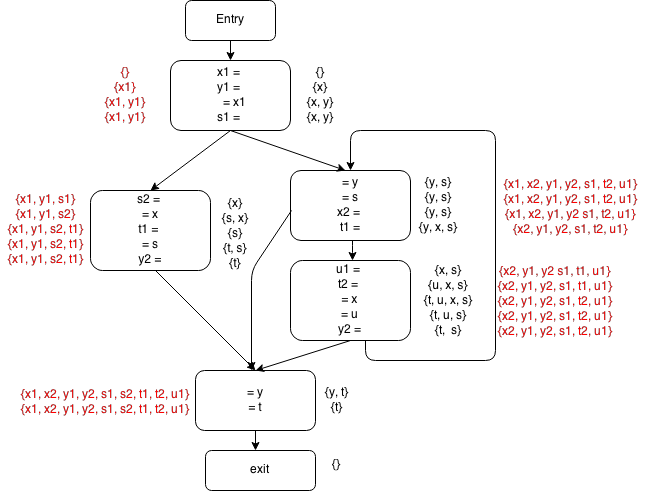
\includegraphics[scale=0.6]{1.png}
\end{center}

\item Create the interference graph:
\begin{center}
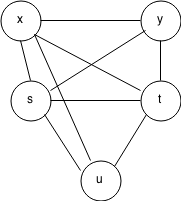
\includegraphics[scale=0.6]{2.png}
\end{center}
\item Perform coloring and spilling. We are using Chaitin's algorithm here. The
stack we obtain is: $[t, s, y, x, u]$. We then pop the stack and assign
registers as follows: t gets r0, s gets r1, y gets r2, x gets r3 and u gets r2.
We see here that we are able to assign all variables to registers without
spilling.
\end{itemize}
\end{question}
\newpage

\begin{question}{Instruction Scheduling}

The answers to parts 1 and 2 are in the following table:

\begin{tabular}{|c|c|c|c|c|}
\hline
Clock Cycle	&	Ready(forwards)	&	Issued(forwards)	&	Ready(backwards)	&	Issued(backwards)\\
\hline
0			&	(1, 2, 4)			&	(1)				&	(1, 2, 4)			&	(1)				\\
\hline
1			&	(2, 4)				&	(2)				&	(2, 4)				&	(2)				\\
\hline
2			&	(4)				&	(4)				&	(4)				&	()				\\
\hline
3			&	()				&	()				&	(4)				&	(4)				\\
\hline
4			&	(3, 5)				&	(3, 5)				&	(3, 5)				&	(5)				\\
\hline
5			&	(6, 7, 9, 10)		&	(6, 7)				&	(3, 7, 9)			&	(7)				\\
\hline
6			&	(8, 9, 10)			&	(9, 10)			&	(3, 6, 8, 9, 10)		&	(6, 10)			\\
\hline
7			&	(8)				&	(8)				&	(3, 8, 9)			&	(8, 9)				\\
\hline
8			&	(12)				&	(12)				&	(3)				&	(3)				\\
\hline
9			&	()				&	()				&	(12)				&	()				\\
\hline
10			&	(11, 13)			&	(11, 13)			&	(11, 12)			&	(12)				\\
\hline
11			&	(14)				&	(14)				&	(11, 13)			&	(11, 13)			\\
\hline
12			&	(15)				&	(15)				&	(14)				&	(14)				\\
\hline
13			&					&					&	(15)				&	(15)				\\
\hline
\end{tabular}

\end{question}
\end{document}
